\documentclass[aspectratio=169, 10pt]{beamer}

% ---------------------------------------------------------------------------
%  Theme & colours
% ---------------------------------------------------------------------------
\usetheme{Madrid}
\usecolortheme{beaver}

\setbeamertemplate{navigation symbols}{}          % remove nav icons
\setbeamertemplate{footline}{%
  \leavevmode%
  \hbox{%
    \begin{beamercolorbox}[wd=.33\paperwidth,ht=2.25ex,dp=1ex,center]{author in head/foot}%
      \usebeamerfont{author in head/foot}Kasra
    \end{beamercolorbox}%
    \begin{beamercolorbox}[wd=.34\paperwidth,ht=2.25ex,dp=1ex,center]{title in head/foot}%
      \usebeamerfont{title in head/foot}MoA Prediction
    \end{beamercolorbox}%
    \begin{beamercolorbox}[wd=.33\paperwidth,ht=2.25ex,dp=1ex,right]{date in head/foot}%
      \usebeamerfont{date in head/foot}\insertframenumber{} / \inserttotalframenumber\hspace*{2ex}
    \end{beamercolorbox}}%
}

% ---------------------------------------------------------------------------
%  Packages
% ---------------------------------------------------------------------------
\usepackage[utf8]{inputenc}
\usepackage{amsmath, amssymb}
\usepackage{booktabs}
\usepackage{xcolor}
\usepackage{tikz}
\usetikzlibrary{shapes.geometric, arrows.meta, positioning, fit, backgrounds}
\usepackage{array}
\usepackage{colortbl}
\usepackage{graphicx}
\usepackage{listings}

% ---------------------------------------------------------------------------
%  Custom colours
% ---------------------------------------------------------------------------
\definecolor{darkred}{RGB}{160,20,20}
\definecolor{midblue}{RGB}{30,80,160}
\definecolor{lightgray}{RGB}{240,240,240}
\definecolor{darkorange}{RGB}{200,100,0}
\definecolor{darkgreen}{RGB}{0,120,50}
\definecolor{mygray}{RGB}{245,245,245}

% Highlight box
\newcommand{\hilight}[1]{\colorbox{yellow!35}{#1}}

% ---------------------------------------------------------------------------
%  Meta
% ---------------------------------------------------------------------------
\title[MoA Prediction]{%
  \textbf{Mechanisms of Action (MoA) Prediction}\\[0.3em]
  {\normalsize Multi-label Drug Classification with Deep Learning}}
\author[Kasra]{Kasra}
\institute[Genomics Project]{Genomics Course Project}
\date{April 2026}

% ===========================================================================
\begin{document}
% ===========================================================================

% ---------------------------------------------------------------------------
%  TITLE
% ---------------------------------------------------------------------------
\begin{frame}
  \titlepage
\end{frame}

% ---------------------------------------------------------------------------
%  OUTLINE
% ---------------------------------------------------------------------------
\begin{frame}{Outline}
  \tableofcontents
\end{frame}

% ===========================================================================
\section{Background}
% ===========================================================================

\begin{frame}{The Competition}
  \begin{columns}[T]
    \begin{column}{0.55\textwidth}
      \textbf{LISH-MoA — Kaggle 2020}\\[0.5em]
      Organised jointly by:
      \begin{itemize}
        \item \textbf{Broad Institute of MIT \& Harvard}\\
              Home of the Connectivity Map project
        \item \textbf{Laboratory for Innovation Science\\
              at Harvard (LISH)}
        \item \textbf{NIH LINCS}\\
              Library of Integrated Network-Based\\
              Cellular Signatures
      \end{itemize}
      \vspace{0.6em}
      Prize pool: \$30,000 \quad|\quad 4,373 teams
    \end{column}
    \begin{column}{0.42\textwidth}
      \begin{block}{Motivation}
        Traditional drug discovery is \textbf{serendipitous}.
        The shift toward targeted medicine requires
        automatically characterising \emph{what a drug does}
        at the molecular level — its \textbf{Mechanism of Action}.
      \end{block}
      \vspace{0.5em}
      \begin{alertblock}{Why it matters}
        Knowing a drug's MoA guides:
        \begin{itemize}
          \item Target identification
          \item Side-effect prediction
          \item Drug repurposing
        \end{itemize}
      \end{alertblock}
    \end{column}
  \end{columns}
\end{frame}

\begin{frame}{What is a Mechanism of Action?}
  \begin{columns}[T]
    \begin{column}{0.52\textwidth}
      A \textbf{Mechanism of Action (MoA)} describes how a drug
      produces its pharmacological effect at the molecular level.
      \vspace{0.8em}

      \textbf{Example:} Ibuprofen inhibits the COX-1 and COX-2
      enzymes, which reduces prostaglandin synthesis,
      leading to anti-inflammatory effects.
      \vspace{0.8em}

      \textbf{How to determine MoA experimentally:}
      \begin{enumerate}
        \item Treat human cells with the drug
        \item Measure gene expression response
        \item Measure cell viability response
        \item Match response patterns to known MoA libraries
      \end{enumerate}
    \end{column}
    \begin{column}{0.44\textwidth}
      \begin{exampleblock}{Our Approach}
        Instead of manually matching patterns, we train a neural
        network to \textbf{automatically predict} which MoA labels
        are active, given the measured cellular response.
      \end{exampleblock}
      \vspace{0.6em}
      \begin{block}{Key novelty of this dataset}
        Responses are measured \textbf{simultaneously across
        100 cell types} using a new pooled technology —
        removing the need to pre-select which cell type
        to use for a given drug.
      \end{block}
    \end{column}
  \end{columns}
\end{frame}

\begin{frame}{Project Goal}
  \begin{center}
    \Large
    Given gene expression and cell viability measurements\\[0.4em]
    for a drug-treated sample,\\[0.6em]
    \textbf{predict which of 206 binary MoA labels are active.}
  \end{center}
  \vspace{0.5em}
  \begin{columns}[T]
    \begin{column}{0.48\textwidth}
      \begin{block}{Formal task}
        \textbf{Multi-label binary classification}\\[0.3em]
        Input: $\mathbf{x} \in \mathbb{R}^{1560}$\\[0.2em]
        Output: $\hat{\mathbf{y}} \in [0,1]^{206}$\\[0.2em]
        Each $\hat{y}_m$ is the probability that MoA $m$ is active.
      \end{block}
    \end{column}
    \begin{column}{0.48\textwidth}
      \begin{alertblock}{Three core challenges}
        \begin{enumerate}
          \item \textbf{Extreme class imbalance}\\
                Mean positive rate: $0.34\%$
          \item \textbf{High dimensionality}\\
                876 raw features, redundant
          \item \textbf{Drug leakage in CV}\\
                Same drug $\to$ multiple samples
        \end{enumerate}
      \end{alertblock}
    \end{column}
  \end{columns}
\end{frame}

% ===========================================================================
\section{Dataset}
% ===========================================================================

\begin{frame}{Dataset Overview}
  \begin{columns}[T]
    \begin{column}{0.5\textwidth}
      \begin{table}
        \caption{Files and dimensions}
        \small
        \begin{tabular}{lrr}
          \toprule
          \textbf{File} & \textbf{Rows} & \textbf{Cols} \\
          \midrule
          train\_features  & 23,814 & 876 \\
          test\_features   & 3,982  & 876 \\
          targets\_scored  & 23,814 & 207 \\
          targets\_nonscored & 23,814 & 403 \\
          train\_drug      & 23,814 & 2   \\
          \bottomrule
        \end{tabular}
      \end{table}
      \vspace{0.5em}
      \textbf{Feature breakdown (876 columns):}
      \begin{itemize}
        \item 4 metadata columns
        \item \textbf{772} gene expression features (\texttt{g-0} \ldots \texttt{g-771})
        \item \textbf{100} cell viability features (\texttt{c-0} \ldots \texttt{c-99})
      \end{itemize}
    \end{column}
    \begin{column}{0.47\textwidth}
      \begin{block}{Metadata columns}
        \begin{itemize}
          \item \texttt{sig\_id} — sample identifier
          \item \texttt{cp\_type} — \texttt{trt\_cp} or \texttt{ctl\_vehicle}
          \item \texttt{cp\_time} — 24 / 48 / 72 hours
          \item \texttt{cp\_dose} — D1 (low) or D2 (high)
        \end{itemize}
      \end{block}
      \vspace{0.4em}
      \begin{alertblock}{Control samples}
        \texttt{ctl\_vehicle} samples receive \textbf{no drug}.\\
        All 206 MoA labels are always \textbf{zero} for controls.\\[0.3em]
        Train: 1,866 controls ($7.8\%$)\\
        Test: \phantom{1,}358 controls ($9.0\%$)
      \end{alertblock}
    \end{column}
  \end{columns}
\end{frame}

\begin{frame}{The Class Imbalance Problem}
  \begin{columns}[T]
    \begin{column}{0.48\textwidth}
      \begin{table}
        \caption{Positive rate across 206 scored targets}
        \small
        \begin{tabular}{lr}
          \toprule
          \textbf{Statistic} & \textbf{Value} \\
          \midrule
          Minimum & $0.004\%$ \\
          Median  & $0.162\%$ \\
          Mean    & $0.343\%$ \\
          Maximum & $3.494\%$ \\
          \midrule
          Targets $<0.5\%$ positive & 173 / 206 \\
          Targets $<1.0\%$ positive & 184 / 206 \\
          Targets $>1.0\%$ positive & 22 / 206  \\
          Targets $>3.0\%$ positive & 2 / 206   \\
          \bottomrule
        \end{tabular}
      \end{table}
    \end{column}
    \begin{column}{0.48\textwidth}
      \begin{alertblock}{Why this is hard}
        For the most common target (3.5\%), a model that
        \textbf{always predicts zero} still gets $96.5\%$ of
        that column right.\\[0.5em]
        For targets below $0.1\%$ positive rate,
        the model sees fewer than 25 positive examples
        in the entire training set of 23,814 rows.
      \end{alertblock}
      \vspace{0.4em}
      \begin{exampleblock}{Consequence}
        Accuracy is useless as a metric.\\
        The model needs \textbf{calibrated probabilities},
        not hard predictions.
      \end{exampleblock}
    \end{column}
  \end{columns}
\end{frame}

% ===========================================================================
\section{Data Processing}
% ===========================================================================

\begin{frame}{Cross-Validation: Drug-Level Grouping}
  \begin{columns}[T]
    \begin{column}{0.5\textwidth}
      \textbf{The leakage problem:}\\[0.3em]
      Each drug appears in \textbf{multiple samples}
      (different dose $\times$ time combinations).
      A naive sample-level split places the same drug in
      both train and validation, inflating scores.

      \vspace{0.6em}
      \textbf{Correct approach:}
      \begin{enumerate}
        \item Aggregate targets to drug level
        \item Stratify and split \emph{drugs} into 5 folds
        \item Map drug fold assignments back to samples
        \item Validation fold = samples from drugs the model
              has never seen
      \end{enumerate}
    \end{column}
    \begin{column}{0.46\textwidth}
      \begin{block}{MultilabelStratifiedKFold}
        Ensures each fold has a representative distribution
        of positive rates for all 206 targets.\\[0.4em]
        Used in \textbf{both} Experiment 1 and 2.
      \end{block}
      \vspace{0.5em}
      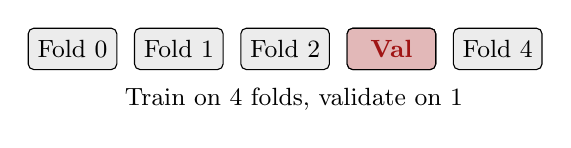
\begin{tikzpicture}[scale=0.75, font=\small]
        \foreach \i in {0,...,4} {
          \draw[fill=gray!15, rounded corners=2pt]
            (\i*1.8, 0) rectangle (\i*1.8+1.5, 0.7);
          \node at (\i*1.8+0.75, 0.35) {Fold \i};
        }
        \draw[fill=darkred!30, rounded corners=2pt]
          (3*1.8, 0) rectangle (3*1.8+1.5, 0.7);
        \node[darkred] at (3*1.8+0.75, 0.35) {\textbf{Val}};
        \node at (4.5, -0.5) {\small Train on 4 folds, validate on 1};
      \end{tikzpicture}
    \end{column}
  \end{columns}
\end{frame}

\begin{frame}{Data Processing — Experiment 1 vs Experiment 2}
  \begin{columns}[T]
    \begin{column}{0.48\textwidth}
      \textbf{\color{darkred}Experiment 1 (Minimal)}
      \begin{itemize}
        \item Remove control samples from training
        \item \texttt{cp\_dose} $\to$ binary 0/1
        \item \texttt{cp\_time} passed as raw integer
        \item Gene and cell features: \textbf{no normalisation}
        \item Input dim: \textbf{873}
      \end{itemize}
      \vspace{0.4em}
      \textit{Raw, unnormalised features go directly into the network.}
    \end{column}
    \begin{column}{0.48\textwidth}
      \textbf{\color{midblue}Experiment 2 (Full Pipeline)}
      \begin{itemize}
        \item Metadata: \texttt{cp\_type}, \texttt{cp\_time}/72, \texttt{cp\_dose}
        \item \textbf{QuantileTransformer} (Gaussian output) on gene and cell features separately
        \item \textbf{PCA} (95\% variance) on gene and cell features separately
        \item Concatenate: QT features + PCA features
        \item Input dim: \textbf{1,560}
      \end{itemize}
      \[
        \underbrace{3}_{\text{meta}}
        + \underbrace{602}_{\text{gene PCA}}
        + \underbrace{83}_{\text{cell PCA}}
        + \underbrace{772}_{\text{gene QT}}
        + \underbrace{100}_{\text{cell QT}}
        = 1560
      \]
    \end{column}
  \end{columns}

  \vspace{0.5em}
  \begin{exampleblock}{Why QuantileTransformer?}
    Gene expression assays produce outliers. QT maps any empirical distribution to
    $\mathcal{N}(0,1)$, making the feature scales uniform and matching the
    assumptions of batch normalisation. Fit on train only to prevent leakage.
  \end{exampleblock}
\end{frame}

% ===========================================================================
\section{Evaluation Metric}
% ===========================================================================

\begin{frame}{Evaluation Metric: Mean Column-wise Log Loss}
  \begin{block}{Competition metric (lower is better)}
    \[
      \mathcal{L}_{\text{MoA}} =
      -\frac{1}{M} \sum_{m=1}^{M}
      \frac{1}{N} \sum_{i=1}^{N}
      \Bigl[
        y_{i,m} \log \hat{y}_{i,m}
        + (1 - y_{i,m}) \log(1 - \hat{y}_{i,m})
      \Bigr]
    \]
    $M = 206$ targets, $N$ samples. Average log loss \textbf{per column}, then average across columns.
  \end{block}

  \vspace{0.4em}
  \textbf{Key properties:}
  \begin{itemize}
    \item \textbf{Equal weight per column} — a target with $0.04\%$ positives counts
          the same as the most common target ($3.5\%$). Every column must be predicted well.
    \item \textbf{Severely penalises confident wrong answers}:
          predicting $\hat{y} = 0.01$ for a true positive $\Rightarrow$ loss $\approx 4.6$;
          predicting $\hat{y} = 0.5$ $\Rightarrow$ loss $\approx 0.69$.
    \item \textbf{Requires calibrated probabilities}, not binary predictions.
  \end{itemize}
\end{frame}

\begin{frame}{Log Loss vs BCE Loss — What is the Difference?}
  \begin{columns}[T]
    \begin{column}{0.48\textwidth}
      \begin{block}{BCE Loss (used in training)}
        \[
          \mathcal{L}_{\text{BCE}} =
          -\frac{1}{N \cdot M}
          \sum_{i,m} \bigl[ y_{i,m} \log \hat{y}_{i,m}
          + \ldots \bigr]
        \]
        Average over \textbf{all $N \times M$ cells jointly}.\\[0.4em]
        Rare targets contribute proportionally less — their
        many-zero cells get diluted in the global average.
      \end{block}
    \end{column}
    \begin{column}{0.48\textwidth}
      \begin{block}{MoA Log Loss (competition)}
        \[
          \mathcal{L}_{\text{MoA}} =
          \frac{1}{M} \sum_m
          \underbrace{\frac{1}{N} \sum_i \bigl[\ldots\bigr]}_{\text{per-column loss}}
        \]
        Average \textbf{within each column first}, then across
        columns.\\[0.4em]
        Every MoA gets equal weight regardless of frequency.
      \end{block}
    \end{column}
  \end{columns}

  \vspace{0.5em}
  \begin{alertblock}{Practical consequence}
    A model can achieve low BCE loss by ignoring rare targets (predicting near-zero
    everywhere). The competition metric will expose this — rare targets that are
    poorly calibrated pull the score up just as much as common ones.\\[0.3em]
    \textbf{Experiment 1 only tracked BCE. We add the competition metric in Experiment 2.}
  \end{alertblock}
\end{frame}

\begin{frame}{Reference Baselines}
  \begin{table}
    \caption{Score reference points (MoA log loss, lower is better)}
    \begin{tabular}{lcc}
      \toprule
      \textbf{Strategy} & \textbf{MoA Log Loss} & \textbf{Notes} \\
      \midrule
      Predict 0.5 everywhere      & $\sim 0.693$ & Pure ignorance \\
      Predict column-mean pos rate & $\sim 0.022$ & Trivial baseline \\
      \rowcolor{yellow!25}
      Experiment 1 (baseline MLP) & $\sim 0.021$ & Est.\ from BCE \\
      \rowcolor{green!15}
      Experiment 2 (improved MLP) & TBD          & After full run \\
      Kaggle top leaderboard      & $\sim 0.013$ & Ensemble of many models \\
      \bottomrule
    \end{tabular}
  \end{table}

  \vspace{0.4em}
  \begin{exampleblock}{Critical threshold}
    Any model that scores \textbf{worse than $\sim 0.022$} provides no useful
    information beyond knowing the prior positive rates.
    This is the minimum bar to clear.
  \end{exampleblock}
\end{frame}

% ===========================================================================
\section{Models}
% ===========================================================================

\begin{frame}{Experiment 1 — Baseline MLP}
  \begin{columns}[T]
    \begin{column}{0.44\textwidth}
      \textbf{Architecture:}\\[0.4em]
      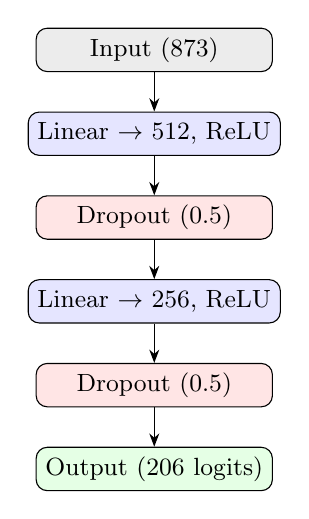
\begin{tikzpicture}[font=\small, node distance=0.5cm]
        \node[draw, fill=gray!15, rounded corners, minimum width=3cm, minimum height=0.55cm]
          (inp) {Input (873)};
        \node[draw, fill=blue!10, rounded corners, minimum width=3cm, minimum height=0.55cm,
              below=of inp] (h1) {Linear $\to$ 512, ReLU};
        \node[draw, fill=red!10, rounded corners, minimum width=3cm, minimum height=0.55cm,
              below=of h1] (d1) {Dropout (0.5)};
        \node[draw, fill=blue!10, rounded corners, minimum width=3cm, minimum height=0.55cm,
              below=of d1] (h2) {Linear $\to$ 256, ReLU};
        \node[draw, fill=red!10, rounded corners, minimum width=3cm, minimum height=0.55cm,
              below=of h2] (d2) {Dropout (0.5)};
        \node[draw, fill=green!10, rounded corners, minimum width=3cm, minimum height=0.55cm,
              below=of d2] (out) {Output (206 logits)};
        \foreach \a/\b in {inp/h1, h1/d1, d1/h2, h2/d2, d2/out}
          \draw[-Stealth] (\a) -- (\b);
      \end{tikzpicture}
    \end{column}
    \begin{column}{0.52\textwidth}
      \textbf{Training setup:}
      \begin{itemize}
        \item Optimiser: Adam, lr = $10^{-3}$
        \item Loss: BCEWithLogitsLoss (no smoothing)
        \item Batch size: 128, Epochs: 50 (fixed)
        \item No LR schedule, no early stopping
      \end{itemize}
      \vspace{0.5em}
      \begin{alertblock}{Problems observed}
        \begin{itemize}
          \item \textbf{Severe overfitting}: Train F1 $\to 0.60$, Val F1 stays $< 0.08$
          \item Val loss rises from epoch $\sim$10 onward
          \item No mechanism to stop early
          \item Wrong metric tracked (F1, not log loss)
          \item 402 non-scored targets completely ignored
        \end{itemize}
      \end{alertblock}
    \end{column}
  \end{columns}
\end{frame}

\begin{frame}{From Experiment 1 to Experiment 2 — Design Decisions}
  \begin{table}
    \small
    \begin{tabular}{lll}
      \toprule
      \textbf{Aspect} & \textbf{Exp 1} & \textbf{Exp 2 (fix \& why)} \\
      \midrule
      Feature normalisation & None & QuantileTransformer — outlier robustness \\
      Dimensionality & 873 raw & 1560 (QT + PCA) — cleaner signal \\
      Batch normalisation & No & Yes — stable gradients, allows depth \\
      Activation & ReLU & SiLU — smooth, no dying neurons \\
      Residual connections & No & Yes — shortcuts gradient, adds depth \\
      Dropout & 0.5 & 0.3 — BN already regularises \\
      Weight init & Default & Kaiming — variance stability \\
      Multi-task targets & 206 & 206 + 402 — free regularisation signal \\
      Optimiser & Adam & AdamW — proper weight decay \\
      LR schedule & None & Cosine annealing — better convergence \\
      Label smoothing & No & $\varepsilon=0.001$ — calibration, prevents overconfidence \\
      Early stopping & No & Patience 15 — stops overfitting \\
      Tracked metric & BCE, F1 & MoA log loss — competition metric \\
      \bottomrule
    \end{tabular}
  \end{table}
\end{frame}

\begin{frame}{Experiment 2 — Improved BN-MLP Architecture}
  \begin{columns}[T]
    \begin{column}{0.5\textwidth}
      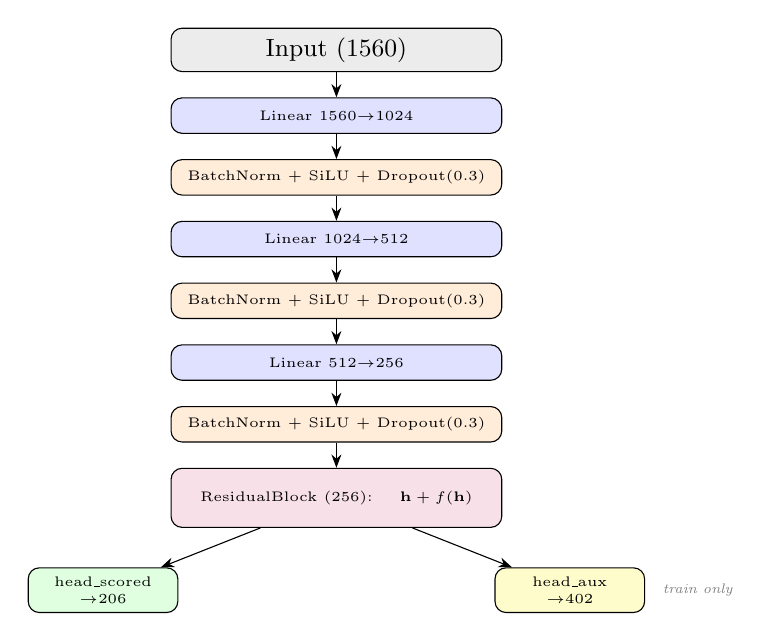
\begin{tikzpicture}[font=\tiny, node distance=0.32cm]
        \node[draw, fill=gray!15, rounded corners, minimum width=4.2cm, minimum height=0.5cm]
          (inp) {\small Input (1560)};

        \node[draw, fill=blue!12, rounded corners, minimum width=4.2cm, minimum height=0.45cm,
              below=of inp] (l1) {Linear 1560$\to$1024};
        \node[draw, fill=orange!15, rounded corners, minimum width=4.2cm, minimum height=0.45cm,
              below=of l1] (b1) {BatchNorm + SiLU + Dropout(0.3)};

        \node[draw, fill=blue!12, rounded corners, minimum width=4.2cm, minimum height=0.45cm,
              below=of b1] (l2) {Linear 1024$\to$512};
        \node[draw, fill=orange!15, rounded corners, minimum width=4.2cm, minimum height=0.45cm,
              below=of l2] (b2) {BatchNorm + SiLU + Dropout(0.3)};

        \node[draw, fill=blue!12, rounded corners, minimum width=4.2cm, minimum height=0.45cm,
              below=of b2] (l3) {Linear 512$\to$256};
        \node[draw, fill=orange!15, rounded corners, minimum width=4.2cm, minimum height=0.45cm,
              below=of l3] (b3) {BatchNorm + SiLU + Dropout(0.3)};

        \node[draw, fill=purple!12, rounded corners, minimum width=4.2cm, minimum height=0.75cm,
              below=of b3] (res) {ResidualBlock (256): \quad $\mathbf{h} + f(\mathbf{h})$};

        \node[draw, fill=green!12, rounded corners, align=center, minimum width=1.9cm, minimum height=0.5cm,
              below left=0.5cm and -0.1cm of res] (hs) {head\_scored\\$\to$206};
        \node[draw, fill=yellow!20, rounded corners, align=center, minimum width=1.9cm, minimum height=0.5cm,
              below right=0.5cm and -0.1cm of res] (ha) {head\_aux\\$\to$402};

        \foreach \a/\b in {inp/l1, l1/b1, b1/l2, l2/b2, b2/l3, l3/b3, b3/res}
          \draw[-Stealth] (\a) -- (\b);
        \draw[-Stealth] (res) -- (hs);
        \draw[-Stealth] (res) -- (ha);

        \node[right=0.1cm of ha, text=gray, font=\tiny\itshape]
          (tr) {train only};
      \end{tikzpicture}
    \end{column}
    \begin{column}{0.46\textwidth}
      \textbf{BatchNorm} — stabilises gradient magnitudes;\\
      allows greater depth without saturation.\\[0.4em]
      \textbf{SiLU}: $x \cdot \sigma(x)$ — smooth, non-monotonic;\\
      no dying neurons; better than ReLU on bio data.\\[0.4em]
      \textbf{ResidualBlock}: skip connection $\mathbf{h} + f(\mathbf{h})$;\\
      adding depth cannot hurt; shorter gradient path.\\[0.4em]
      \textbf{Dual heads / Multi-task}:\\
      402 non-scored labels share the same biology.
      Training on both forces the backbone to learn
      a richer, more general representation.
      Auxiliary head is discarded at inference.\\[0.4em]
      \textbf{Kaiming init}: $W \sim \mathcal{N}(0,\sqrt{2/\text{fan\_in}})$\\
      Keeps activation variance stable at init.
    \end{column}
  \end{columns}
\end{frame}

\begin{frame}{Experiment 2 — Training Strategy}
  \begin{columns}[T]
    \begin{column}{0.48\textwidth}
      \begin{block}{Optimiser: AdamW}
        Decouples weight decay from the gradient update:\\
        $\theta \leftarrow \theta - \alpha \hat{m}/(\sqrt{\hat{v}}+\epsilon) - \alpha\lambda\theta$\\[0.3em]
        Standard Adam's L2 penalty is scaled by the adaptive
        LR, weakening it on high-gradient parameters.
        AdamW fixes this.
      \end{block}
      \vspace{0.4em}
      \begin{block}{Label Smoothing ($\varepsilon = 0.001$)}
        \[ \tilde{y} = y(1-\varepsilon) + 0.5\varepsilon \]
        Prevents logits from collapsing to $\pm\infty$.
        Especially important for the severely imbalanced
        negative class — stops overconfident zero predictions.
      \end{block}
    \end{column}
    \begin{column}{0.48\textwidth}
      \begin{block}{Cosine Annealing}
        \[ \eta_t = \eta_{\min} + \tfrac{1}{2}(\eta_{\max}-\eta_{\min})
           \!\left(1+\cos\tfrac{\pi t}{T_{\max}}\right) \]
        Large steps early (exploration), fine-grained
        refinement near convergence.
      \end{block}
      \vspace{0.4em}
      \begin{block}{Total Loss}
        \[ \mathcal{L} = \mathcal{L}_{\text{scored}} +
           \underbrace{0.3}_{\lambda_{\text{aux}}} \cdot \mathcal{L}_{\text{aux}} \]
        Auxiliary weight 0.3: enough to regularise,
        not enough to dominate.
      \end{block}
      \vspace{0.3em}
      \textbf{Early stopping:} patience = 15 epochs on val BCE.\\
      \textbf{Gradient clipping:} global norm $\leq 1.0$.
    \end{column}
  \end{columns}
\end{frame}

% ===========================================================================
\section{Results}
% ===========================================================================

\begin{frame}{Results — Experiment 1}
  \begin{columns}[T]
    \begin{column}{0.5\textwidth}
      \begin{table}
        \caption{Per-fold results (Exp 1)}
        \small
        \begin{tabular}{ccc}
          \toprule
          \textbf{Fold} & \textbf{Best Val BCE} & \textbf{Best Val F1} \\
          \midrule
          0 & 0.0206 & 0.0839 \\
          1 & 0.0191 & 0.0770 \\
          2 & 0.0227 & 0.0685 \\
          3 & 0.0186 & 0.0800 \\
          4 & 0.0227 & 0.0711 \\
          \midrule
          \textbf{Mean} & \textbf{0.0207} & \textbf{0.0761} \\
          \bottomrule
        \end{tabular}
      \end{table}
      \vspace{0.3em}
      OOF Macro F1: \textbf{0.0406} \quad OOF Accuracy: \textbf{99.64\%}
    \end{column}
    \begin{column}{0.46\textwidth}
      \begin{alertblock}{Overfitting — epoch 50}
        \begin{itemize}
          \item Train F1: $\mathbf{0.60}$ \quad Val F1: $\mathbf{0.08}$
          \item Train loss still falling at epoch 50
          \item Val loss rising from epoch $\sim$10
        \end{itemize}
      \end{alertblock}
      \vspace{0.4em}
      \begin{exampleblock}{Interpretation}
        High accuracy (99.6\%) is misleading —
        achieved by predicting near-zero everywhere.\\[0.3em]
        The model barely beats the trivial baseline
        ($\sim 0.022$ log loss) estimated from BCE.
      \end{exampleblock}
    \end{column}
  \end{columns}
\end{frame}

\begin{frame}{Results — Experiment 2 (Smoke Test \& Expectations)}
  \begin{columns}[T]
    \begin{column}{0.48\textwidth}
      \begin{block}{2-epoch validation (untrained $\to$ epoch 2)}
        \begin{itemize}
          \item Epoch 0 (random init): log loss $= 0.059$
          \item Epoch 2: log loss $= \mathbf{0.026}$
        \end{itemize}
        Already competitive with Exp 1's \textbf{best checkpoint}
        after just 2 of 100 epochs.
      \end{block}
      \vspace{0.5em}
      \begin{block}{Comparative summary}
        \small
        \begin{tabular}{lcc}
          \toprule
          & \textbf{Exp 1} & \textbf{Exp 2} \\
          \midrule
          Val BCE (best) & 0.0207 & TBD \\
          OOF Macro F1   & 0.0406 & TBD \\
          OOF Log Loss   & $\sim$0.021 & TBD \\
          Epoch 2 log loss & $\sim$0.030 & \textbf{0.026} \\
          \bottomrule
        \end{tabular}
      \end{block}
    \end{column}
    \begin{column}{0.48\textwidth}
      \begin{exampleblock}{Why Exp 2 converges faster}
        \begin{enumerate}
          \item Quantile-normalised inputs have clean,
                Gaussian-shaped distributions — the network
                sees a more learnable signal from step 1.
          \item BatchNorm keeps activations centred through
                depth — gradients propagate efficiently.
          \item SiLU avoids dead neurons — more neurons
                contribute usefully in early epochs.
          \item Multi-task auxiliary loss provides extra
                gradient signal on top of 206 scored targets.
        \end{enumerate}
      \end{exampleblock}
      Full 5-fold run required for final numbers.
    \end{column}
  \end{columns}
\end{frame}

% ===========================================================================
\section{Takeaways \& Future Work}
% ===========================================================================

\begin{frame}{Key Takeaways}
  \begin{enumerate}
    \setlength\itemsep{0.5em}
    \item \textbf{Track the right metric from the start.}\\
          F1 and accuracy are misleading under extreme class imbalance.
          Mean column-wise log loss is the only metric that reflects
          real performance on this task.

    \item \textbf{Preprocessing matters as much as architecture.}\\
          Moving from raw features to quantile-normalised + PCA features
          alone produced faster, more stable convergence.

    \item \textbf{Batch normalisation is essential at depth.}\\
          Without it, Exp 1 showed aggressive overfitting from epoch 10.
          BN stabilised gradients and allowed a wider, deeper network.

    \item \textbf{Drug-level CV is non-negotiable.}\\
          Sample-level splits inflate scores and give false confidence.
          Any published result without drug-level grouping cannot be
          trusted as a generalisation estimate.

    \item \textbf{Non-scored targets are free signal.}\\
          402 auxiliary labels describe the same biology.
          Ignoring them (Exp 1) wastes a significant regularisation
          opportunity at zero additional data cost.
  \end{enumerate}
\end{frame}

\begin{frame}{Future Work}
  \begin{columns}[T]
    \begin{column}{0.48\textwidth}
      \textbf{Immediate (next experiments):}
      \begin{itemize}
        \item Run Exp 2 to full 5-fold completion
        \item Hyperparameter search (hidden dims, dropout,
              learning rate, label smoothing, aux weight)
        \item Temperature / Platt scaling for better
              probability calibration post-training
        \item Threshold tuning on OOF predictions
      \end{itemize}
      \vspace{0.5em}
      \textbf{Feature engineering:}
      \begin{itemize}
        \item Variance-threshold filter before PCA
              to remove near-zero-variance gene features
        \item Statistical feature interactions
              (gene $\times$ dose, gene $\times$ time)
      \end{itemize}
    \end{column}
    \begin{column}{0.48\textwidth}
      \textbf{Model improvements:}
      \begin{itemize}
        \item \textbf{Ensemble with tree models} (LightGBM, XGBoost)
              — captures feature interactions differently;
              top solutions all used ensembles
        \item \textbf{TabNet} — attention-based tabular model with
              instance-wise feature selection; competitive
              on this exact dataset in published work
        \item \textbf{Rank-normalised ensemble blending} — more
              robust than probability averaging across folds
        \item Deeper residual architectures with more blocks
      \end{itemize}
      \vspace{0.3em}
      \begin{exampleblock}{The gap to close}
        Best known: $\sim 0.013$\\
        Our target: $< 0.018$ (beat col-mean baseline
        by $\geq 20\%$)
      \end{exampleblock}
    \end{column}
  \end{columns}
\end{frame}

% ===========================================================================
\section{Conclusion}
% ===========================================================================

\begin{frame}{Conclusion}
  \begin{columns}[T]
    \begin{column}{0.6\textwidth}
      \begin{block}{What we built}
        \begin{itemize}
          \item End-to-end MoA prediction pipeline:
                data loading, drug-grouped CV, training,
                OOF evaluation, test submission
          \item \textbf{Exp 1}: working baseline MLP that exposed
                overfitting and metric-tracking issues
          \item \textbf{Exp 2}: systematically improved model
                addressing every identified weakness —
                preprocessing, architecture, training strategy,
                and evaluation
        \end{itemize}
      \end{block}
      \vspace{0.4em}
      \begin{block}{Core lesson}
        Deep learning on tabular bio data requires careful
        attention to \textbf{data quality, metric choice,
        and regularisation strategy} — the architecture is
        only one part of the story.
      \end{block}
    \end{column}
    \begin{column}{0.36\textwidth}
      \textbf{Experiment 2 is our recommended foundation} for further development.

      \vspace{0.8em}
      \begin{table}
        \small
        \begin{tabular}{lc}
          \toprule
          \textbf{Target} & \textbf{Score} \\
          \midrule
          Col-mean baseline & 0.022 \\
          Our goal & $<$0.018 \\
          Kaggle top & 0.013 \\
          \bottomrule
        \end{tabular}
      \end{table}

      \vspace{0.8em}
      \textbf{Recommended next step:}\\
      Run Exp 2 fully, then add a LightGBM model and blend predictions.
    \end{column}
  \end{columns}
\end{frame}

% ---------------------------------------------------------------------------
%  FINAL SLIDE
% ---------------------------------------------------------------------------
\begin{frame}[plain]
  \begin{center}
    \vspace{2cm}
    {\LARGE \textbf{Thank you}}\\[1em]
    {\large Questions?}\\[2em]
    \rule{6cm}{0.4pt}\\[0.6em]
    \small
    Code: \texttt{src/exp1.ipynb} \quad \texttt{src/exp2.ipynb}\\
    Report: \texttt{report.tex}\\[0.4em]
    Competition: \href{https://www.kaggle.com/competitions/lish-moa}{kaggle.com/competitions/lish-moa}
  \end{center}
\end{frame}

\end{document}
